\documentclass[a4paper]{report}

\usepackage[english]{babel}
\usepackage{hyperref}
\usepackage[utf8]{inputenc}
\usepackage{vubtitlepage}
\usepackage{todonotes}
\usepackage{color}
\usepackage{tabularx}
\usepackage{listings}
\usepackage{url}
\usepackage{graphicx}
\usepackage{hyperref}
\usepackage{a4wide}
\usepackage[nounderscore]{syntax}

\author{\textit{Group 3}\\ Bennet~Stankidis \& Arno~De~Witte}
\faculty{Faculteit Wetenschappen en Bio-ingenieurswetenschappen}

\title{{\Huge Web Engineering}\\Assignment 3}

\lstset{
language=php,
numbers=left,
frame=single,
columns=flexible,
showstringspaces=true,
tabsize=3,
keepspaces=true,
basicstyle=\ttfamily,
breaklines=true,
  basicstyle=\small\ttfamily,
  keywordstyle=\bf\ttfamily\color[rgb]{0,.3,.7},
  commentstyle=\color[rgb]{0.133,0.545,0.133},
  stringstyle={\color[rgb]{0.75,0.49,0.07}}
}

% Nodig voor nieuwe paragrafen "correct" te laten beginnen
\setlength{\parskip}{\medskipamount}
\setlength{\parindent}{0ex}

\begin{document}
\maketitlepage
\tableofcontents
\clearpage










\section{Introduction}
This report is the result of assignment three of the course Web Engineering. It consists of four major deliverables. The mission statement specification, audience modeling (audience classification and audience characterization), conceptual design (task modeling, information modeling, functional modeling and navigational modeling) and implementation design (site structure Design and presentation design).

The online version of HomelessAngel can be found on the url: \url{www.homelessAngel.be}. To use the website as a homeless person the username and password are both \textbf{homeless}. To experience the website as an Angel the username and password are both \textbf{angel}.













\chapter{Mission statement}
\section{Purpose of the website}
The general purpose of this assignment is to create a website where Belgian homeless people and angels, people who want to help, can find each other. The website is a central place that makes it possible for both parties to get to know each other and help one an other. 

The website also wants to help homeless people without the need of angels. It provides general information, information about other organisations, tips, etc. This could benefit homeless people who possibly are not aware of the existence of many useful information.

An other purpose is to bring more attention to the homeless people in Belgium. By creating this website more and more people could become aware of the hassle of being homeless and they could later help the homeless if they want to do that.

\section{Target audience(s) of the website}
There are two target audiences of the HomelessAngel website. The first and most important audience is the homeless people living in Belgium. The second audience is the angels, in other words the people who are willing to help the homeless. 

\section{Subject of the website}
There are three subjects of the website, namely providing information, goods, services and donations. 

The first is giving information to the homeless that could help them with living on the streets, finding a job, improving their life, etc. 

The second one is providing an interface where goods and services are listed that could help a homeless person. These goods and services are given by the angels. An angels can place goods and services online and a homeless person can browse through the offers and request them. 

The third subject is to make it possible to donate money to the website, without even needing to register to the website. 
\\
The website will on their turn use the donated money to help the homeless. The money will make it possible to organise an event where all the homeless people registered on the website may come collect a lunch package. The website will let its users know where and when the event takes place.











\chapter{Audience Modeling}
\section{Audience Classification}
We identified four different audience classes. There is a visitor, angel, homeless person and administrator. These have a hierarchy as described by figure \ref{fig:classhierarchy}. 

\begin{figure}[htp]
\centering
\includegraphics[scale=0.8]{classhierarchy.png}
\caption{Audience class hierarchy diagram}
\label{fig:classhierarchy}
\end{figure}

\section{Audience Characterization}
Below the functional, information and navigational requirements of the audience classes are listed (if applicable). Note that a registered user can not actually exist in the application. It is an abstract user class, as in practice a registered user will either be a homeless person or an angel.

\subsection{Visitor}
\begin{itemize}
	\item Functional requirements
	\begin{itemize}
		\item Makes a donation
	\end{itemize}
	\item Information requirements
	\begin{itemize}
		\item Views all angels and homeless people
		\item Views offered goods and services
	\end{itemize}
	\item Navigational requirements
	\item Characteristics
	\begin{itemize}
		\item Web experience may vary
		\item Language is English
	\end{itemize}
\end{itemize}

\subsection{Registered User}
\begin{itemize}
	\item Functional requirements
	\begin{itemize}
		\item Registers onto the site
		\item Cancels his or her account
	\end{itemize}
\end{itemize}

\subsection{Homeless person}
\begin{itemize}
	\item Functional requirements
	\begin{itemize}
		\item Searches for goods or services
		\item Requests goods or services
		\item Contacts angels which provide goods or services
		\item Rates angels
		\item Finds general information about shelters, rights and tips
	\end{itemize}
	\item Navigational requirements
	\begin{itemize}
		\item Easy navigation between an angel and his or her offerings
	\end{itemize}
	\item Characteristics
	\begin{itemize}
		\item Haves no address
		\item No home internet connection
		\item Computer skills may vary
	\end{itemize}
\end{itemize}

\subsection{Angel}
\begin{itemize}
	\item Functional requirements
	\begin{itemize}
		\item Provides goods or services
		\item Modifies offers
		\item Is able to communicate with homeless people requesting their offerings
	\end{itemize}
	\item Information requirements
	\begin{itemize}
		\item Browses his or her ratings
	\end{itemize}
	\item Navigational requirements
	\item Characteristics
	\begin{itemize}
		\item Angels can be anyone, no specific characteristics can be defined for this group.
	\end{itemize}
\end{itemize}

\subsection{Administrator}
\begin{itemize}
	\item Functional requirements
	\begin{itemize}
		\item Disables a registered user
		\item Removes offerings
	\end{itemize}
	\item Information requirements
	\begin{itemize}
		\item Browses ratings
	\end{itemize}
	\item Navigational requirements
	\item Characteristics
	\begin{itemize}
		\item Is accustomed to the system
	\end{itemize}
\end{itemize}















\chapter{Conceptual Design}
\section{Task Modeling}
ConcurTaskTrees are found in the following alinea's. They are used to describe the tasks that the web system needs to support. Every CTT consists of a small textual explanation combined with the graphical representation of the CTT itself.

\subsection{Provide good or service}
In figure \ref{fig:CTTAddGood} is shown that an angel can enter a good or service. The system will add the offer to the listing.
\begin{figure}[h]
    \centering
    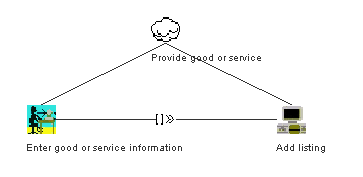
\includegraphics[width=0.8\textwidth]{CTT/CTTpng/CTTAddGood.png}
    \caption{Offer a good or service.}
    \label{fig:CTTAddGood}
\end{figure}

\subsection{Cancel account}
Figure \ref{fig:CTTCancle} depicts how any user, angel or homeless person, can cancel his/her account. 
\begin{figure}[h]
    \centering
    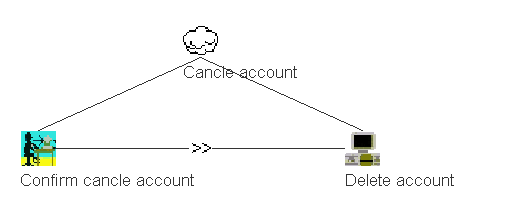
\includegraphics[width=0.8\textwidth]{CTT/CTTpng/CTTCancle.png}
    \caption{Account cancellation.}
    \label{fig:CTTCancle}
\end{figure}

% TODO
% is deze uitleg correct?
% ik vind de naam "Contact Angel" niet zo duidelijk
% want de angel is al gecontacteerd, ik verwachtte dat de CTT toonde hoe ge een angel kon contacteren
\subsection{Contact angel}
Figure \ref{fig:CTTContactAngel} explains how an angel views his/her notification, later pursues it and can have a conversation with the homeless person that sent the message.
\begin{figure}[h]
    \centering
    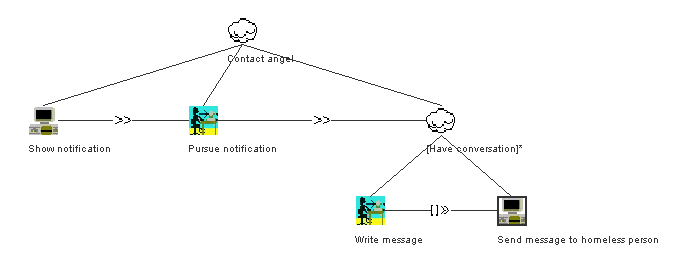
\includegraphics[width=0.8\textwidth]{CTT/CTTpng/CTTContactAngel.png}
    \caption{Angel is contacted and has a conversation.}
    \label{fig:CTTContactAngel}
\end{figure}

\subsection{Contact homeless person}
In figure \ref{fig:CTTContactHomeless} is the same method used as in figure \ref{fig:CTTContactAngel}. In this case the homeless person has a leading role.
\begin{figure}[h]
    \centering
    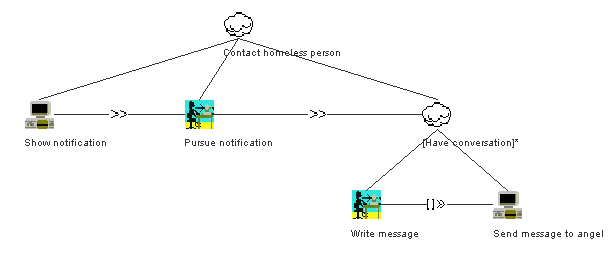
\includegraphics[width=0.8\textwidth]{CTT/CTTpng/CTTContactHomeless.png}
    \caption{Homeless person is contacted and has a conversation.}
    \label{fig:CTTContactHomeless}
\end{figure}

\subsection{Remove offering}
In figure \ref{fig:CTTDeleteOffer} is shown how an angel can delete an offer. An angel can of course only delete offers made by him/her.
\begin{figure}[h]
    \centering
    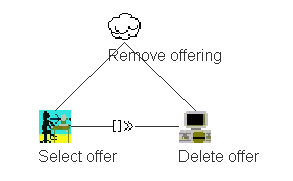
\includegraphics[width=0.8\textwidth]{CTT/CTTpng/CTTDeleteOffer.png}
    \caption{Angel can delete an offer.}
    \label{fig:CTTDeleteOffer}
\end{figure}

\subsection{Disable user}
Figure \ref{fig:CTTDisable} illustrates how an administrator can select a user that will be disabled by the system.
\begin{figure}[h]
    \centering
    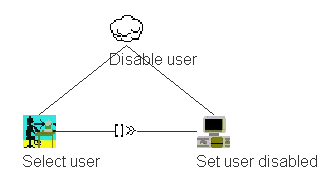
\includegraphics[width=0.8\textwidth]{CTT/CTTpng/CTTDisable.png}
    \caption{Admin disables a user.}
    \label{fig:CTTDisable}
\end{figure}

\subsection{Make a donation}
Figure \ref{fig:CTTDonation} depicts how a visitor of the website can make a donation. The user first needs to specify an amount, then make the payment and after that will the system process the transaction. Important to notify here is that every visitor of the website is able to make a donation. So the visitor, seen in figure \ref{fig:classhierarchy}, is able to help the homeless.
\begin{figure}[h]
    \centering
    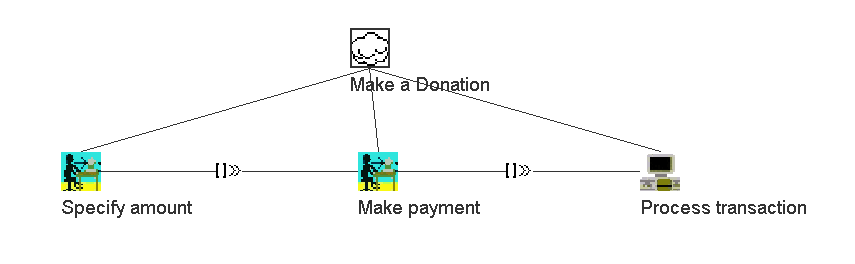
\includegraphics[width=0.8\textwidth]{CTT/CTTpng/CTTDonation.png}
    \caption{Make a donation to help the homeless.}
    \label{fig:CTTDonation}
\end{figure}

% TOOD
% het moet zeker mogelijk zijn om alle offers tegelijk te zien
% is dit een extra mogelijkheid om ze per angel te zien?
\subsection{View offered goods and services}
How a user can view all the offered goods and services of a selected angel is shown in figure \ref{fig:CTTGoods}.
\begin{figure}[h]
    \centering
    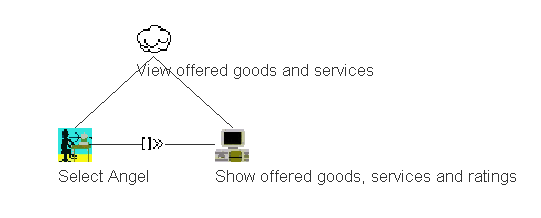
\includegraphics[width=0.8\textwidth]{CTT/CTTpng/CTTGoods.png}
    \caption{View the offers of an angel.}
    \label{fig:CTTGoods}
\end{figure}

% TODO
% hierin zit delete offer
% wat is het verschil met de CTT "Remove offer"?
% TODO
% waarom is [> de relatie tussen modify en delete?
% moet dat niet >> zijn? Want modifying enabled toch niet dat ge kunt deleten?
\subsection{Modify or delete offer}
Figure \ref{fig:CTTModifyOffer} shows how an angel can modify his/her offers. 
\begin{figure}[h]
    \centering
    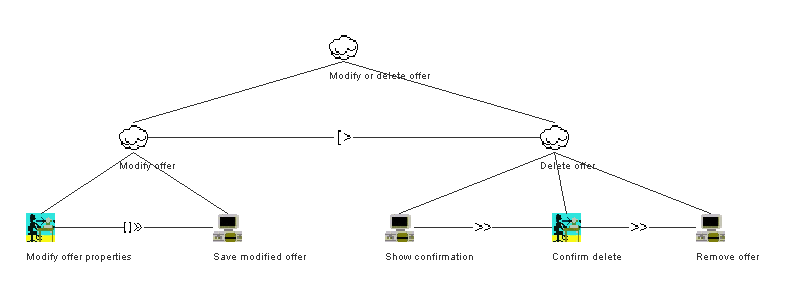
\includegraphics[width=0.8\textwidth]{CTT/CTTpng/CTTModifyOffer.png}
    \caption{Angel can modify or deletes his/her offers.}
    \label{fig:CTTModifyOffer}
\end{figure}

\subsection{Rate Angel}
In figure \ref{fig:CTTRating} is shown how a homeless person can give a rating to an angel. After completing a transaction the homeless person can fill in a rating.
\begin{figure}[h]
    \centering
    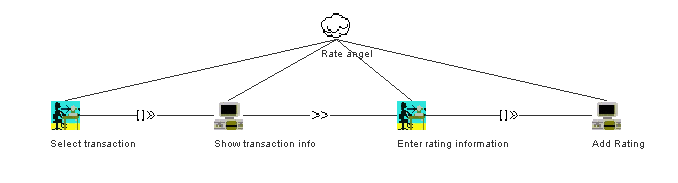
\includegraphics[width=0.8\textwidth]{CTT/CTTpng/CTTRating.png}
    \caption{Rate an angel after a transaction.}
    \label{fig:CTTRating}
\end{figure}

% TODO 
% in de CTT moet eerst de keuze tussen homeless en angel zitten
% adhv die keuze is de personal info anders (wat die info is, moeten we niet tonen)
\subsection{Register account}
Figure \ref{fig:CTTRegister} illustrates how a user can register an account. The user has to fill in personal information to create an account. De personal information depends on the fact dat the new user is an angel or homeless person.
\begin{figure}[h]
    \centering
    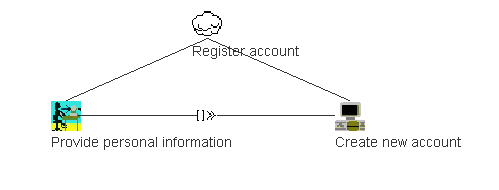
\includegraphics[width=0.8\textwidth]{CTT/CTTpng/CTTRegister.png}
    \caption{Register an account.}
    \label{fig:CTTRegister}
\end{figure}

\subsection{Request goods or services}
Figure \ref{fig:CTTRequestGoods} depicts how a homeless person can select a good of services of interest and then the system creates a new request.
\begin{figure}[h]
    \centering
    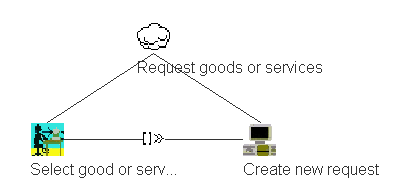
\includegraphics[width=0.8\textwidth]{CTT/CTTpng/CTTRequestGoods.png}
    \caption{Request a good or service of an angel.}
    \label{fig:CTTRequestGoods}
\end{figure}

\subsection{Search goods or services}
Figure \ref{fig:CTTSearchGoods} explains that a homeless person can search on certain keywords to look through the list of offers.
\begin{figure}[h]
    \centering
    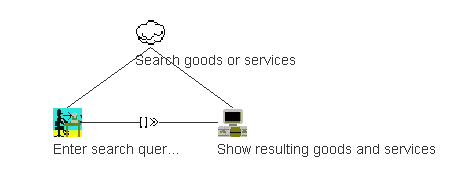
\includegraphics[width=0.8\textwidth]{CTT/CTTpng/CTTSearchGoods.png}
    \caption{Search for certain goods or services.}
    \label{fig:CTTSearchGoods}
\end{figure}

\subsection{View all angels and homeless people}
In figure \ref{fig:awesome_image} is illustrated how a user can view all the registered angels and homeless people. The user is also able to search in the list of all registered users.
\begin{figure}[h]
    \centering
    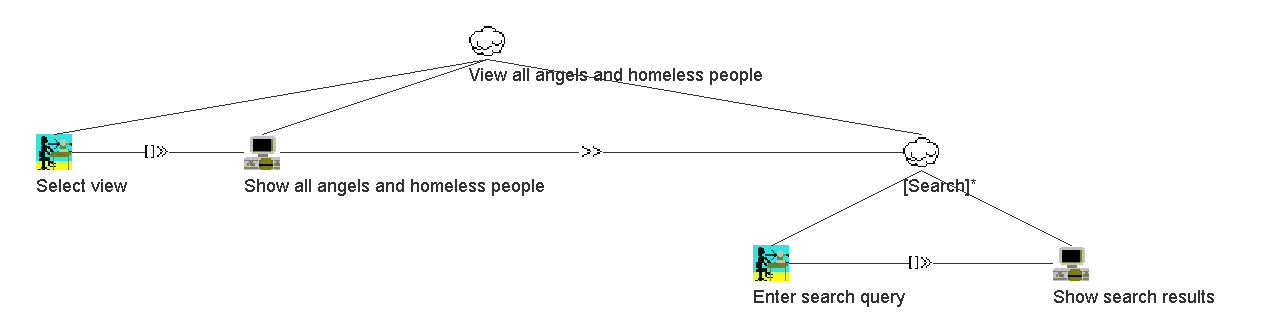
\includegraphics[width=0.8\textwidth]{CTT/CTTpng/CTTViewAngels.png}
    \caption{View all the users and search certain users.}
    \label{fig:CTTViewAngels}
\end{figure}


\section{Information Modeling}
UML

\section{Functional Modeling}
IFML

\section{Navigational Modeling}
IFML












\chapter{Implementation Design}
\section{Site Structure Design}
\section{Presentation Design}
\subsection{Style and Template Design}














\end{document}
